\usetikzlibrary{calc}
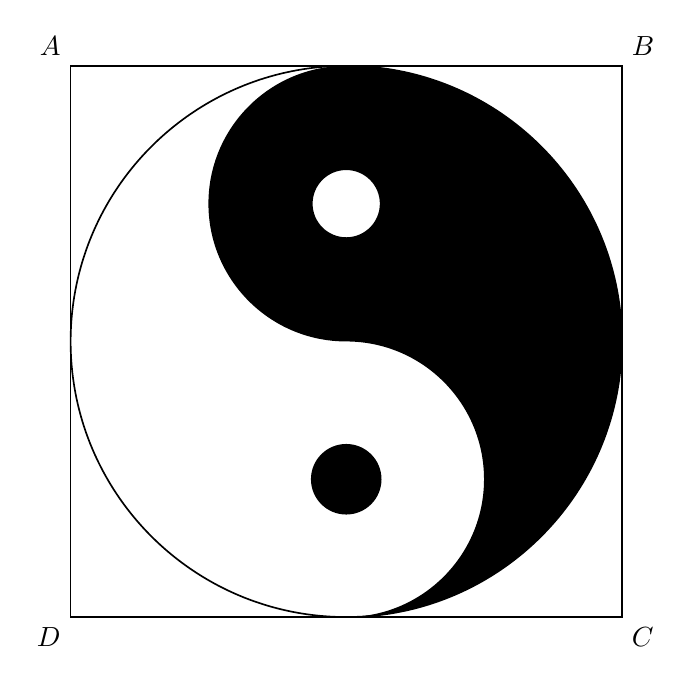
\begin{tikzpicture}[x=1cm,y=1cm,line width=.6pt,font=\normalsize]
\coordinate (O) at (0,0);
\coordinate (U) at (0,1.75);
\coordinate (L) at (0,-1.75);
\coordinate (T) at (0,3.5);
\coordinate (Bm) at (0,-3.5);
\coordinate (Q1) at (-3.5,-3.5);
\coordinate (Q2) at (3.5,-3.5);
\coordinate (Q3) at (3.5,3.5);
\coordinate (Q4) at (-3.5,3.5);
\fill[fill=black,draw=none] (T) arc[start angle=90,delta angle=-180,radius=3.5cm] arc[start angle=270,delta angle=180,radius=1.75cm] arc[start angle=270,delta angle=-180,radius=1.75cm] -- cycle;
\draw (O) circle[radius=3.5cm];
\draw (Q1)--(Q2)--(Q3)--(Q4)--cycle;
\fill[fill=white,draw=black] (U) circle[radius=0.4375cm];
\fill[fill=black,draw=black] (L) circle[radius=0.4375cm];
\node[above left] at (Q4) {$A$};
\node[above right] at (Q3) {$B$};
\node[below right] at (Q2) {$C$};
\node[below left] at (Q1) {$D$};
\end{tikzpicture}
